\documentclass[text06.tex]{subfiles}
\begin{document}
\newpage
\section{Julius}\label{Julius}
次にJuliusを\ruby{紹介}{しょう|かい}します。まずは、たくさんの日本語の言葉の中から、話した言葉を探す音声認識を試してみます。下のようにターミナルにコマンドを入力し、実行しましょう。\\
\mbox{\code{run-linux-gmm.sh}}\\
このコマンドを実行すると、いくらかシステム\ruby{情報}{じょう|ほう}が\ruby{表示}{ひょう|じ}された後、「<<please speak>>」という文字列が\ruby{現}{あらわ}れます（ 図\ref{juliusの使い方}）。
\begin{figure}[H]
\begin{center}
    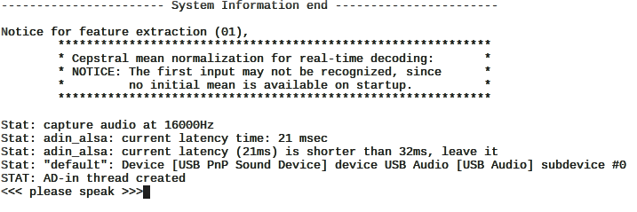
\includegraphics[width=.8\linewidth]{../../asset/image/text06-img009.png}
    \caption{Juliusの使い方}
    \label{juliusの使い方}
\end{center}
\end{figure}
その後マイクに向かって話しかければ、話しかけた単語が文字列になって画面に表示されます。今回は試しに果物の名前を話しかけてみましょう。
\begin{center}
	りんご　みかん　ぶどう　もも　あけび　あんず　いちご　いちじく　かき　スイカ\\すもも　	なし　メロン
\end{center}
\ruby{終了}{しゅう|りょう}するときはCtrl+c（コントロールキーを\ruby{押}{お}しながらcを押す）を使います。<<please speak>>と表示されなくなり、コマンドを入力できる状態になればOKです。

正しく認識することもあれば、\ruby{間違}{ま|ちが}えて認識することもあります。日本語にはたくさんの単語がありますし、\ruby{似}{に}た発音の単語もあるので、それらを\ruby{完璧}{かん|ぺき}に認識することは\ruby{難}{むずか}しいこともあります。次の節では、認識する\ruby{候補}{こう|ほ}の数を変えて、結果を比べてみます。

\begin{tcolorbox}[title=\useOmetoi]
\begin{enumerate}
        \addquiz{ターミナルに\mbox{run-linux-gmm.sh}と入力し、Juliusを試してみましょう。\\<<please speak>>と表示されたらマイクに向かって果物の名前を5つ話しかけましょう。\\たくさんの言葉を認識するとき、5個中何個正しく認識できましたか。}
\end{enumerate}
\end{tcolorbox}
\end{document}
